\documentclass{beamer}
\usepackage[ngerman]{babel}			%Deutsche Umlaute und Umbrüche
\usepackage[utf8]{inputenc}			%utf8 Kodierung
\usepackage{amsmath, amsfonts, amssymb, ulem, epstopdf} %Mathepackete schaden nie
\usetheme{Dresden}
\usecolortheme{beaver}
\usefonttheme{professionalfonts}
\title[TODO]{TODO}
\subtitle{Architectural Document}
\author[C. Stricker\and D. Klopp\and M. Vieth]{Christian Stricker\and David Klopp\and Markus Vieth}
\date[\today]{\today}
\subject{Software engineering}
\newcommand{\btVFill}{\vskip0pt plus 1filll}
\setcounter{tocdepth}{2}
%Link zum Beamer-Userguid: ftp://ftp.dante.de/tex-archive/macros/latex/contrib/beamer/doc/beameruserguide.pdf
\begin{document}
	
	\frame{
		\titlepage
	}
	\setbeamertemplate{footline}[frame number]
	
	\frame[label=IV]{
		\frametitle{Inhaltsverzeichnis}
		\tableofcontents
		[pausesections]
	}
	
	\section[Extern]{Externe Sicht}
	\begin{frame}{Externe Sicht}
		\begin{figure}
			\centering
			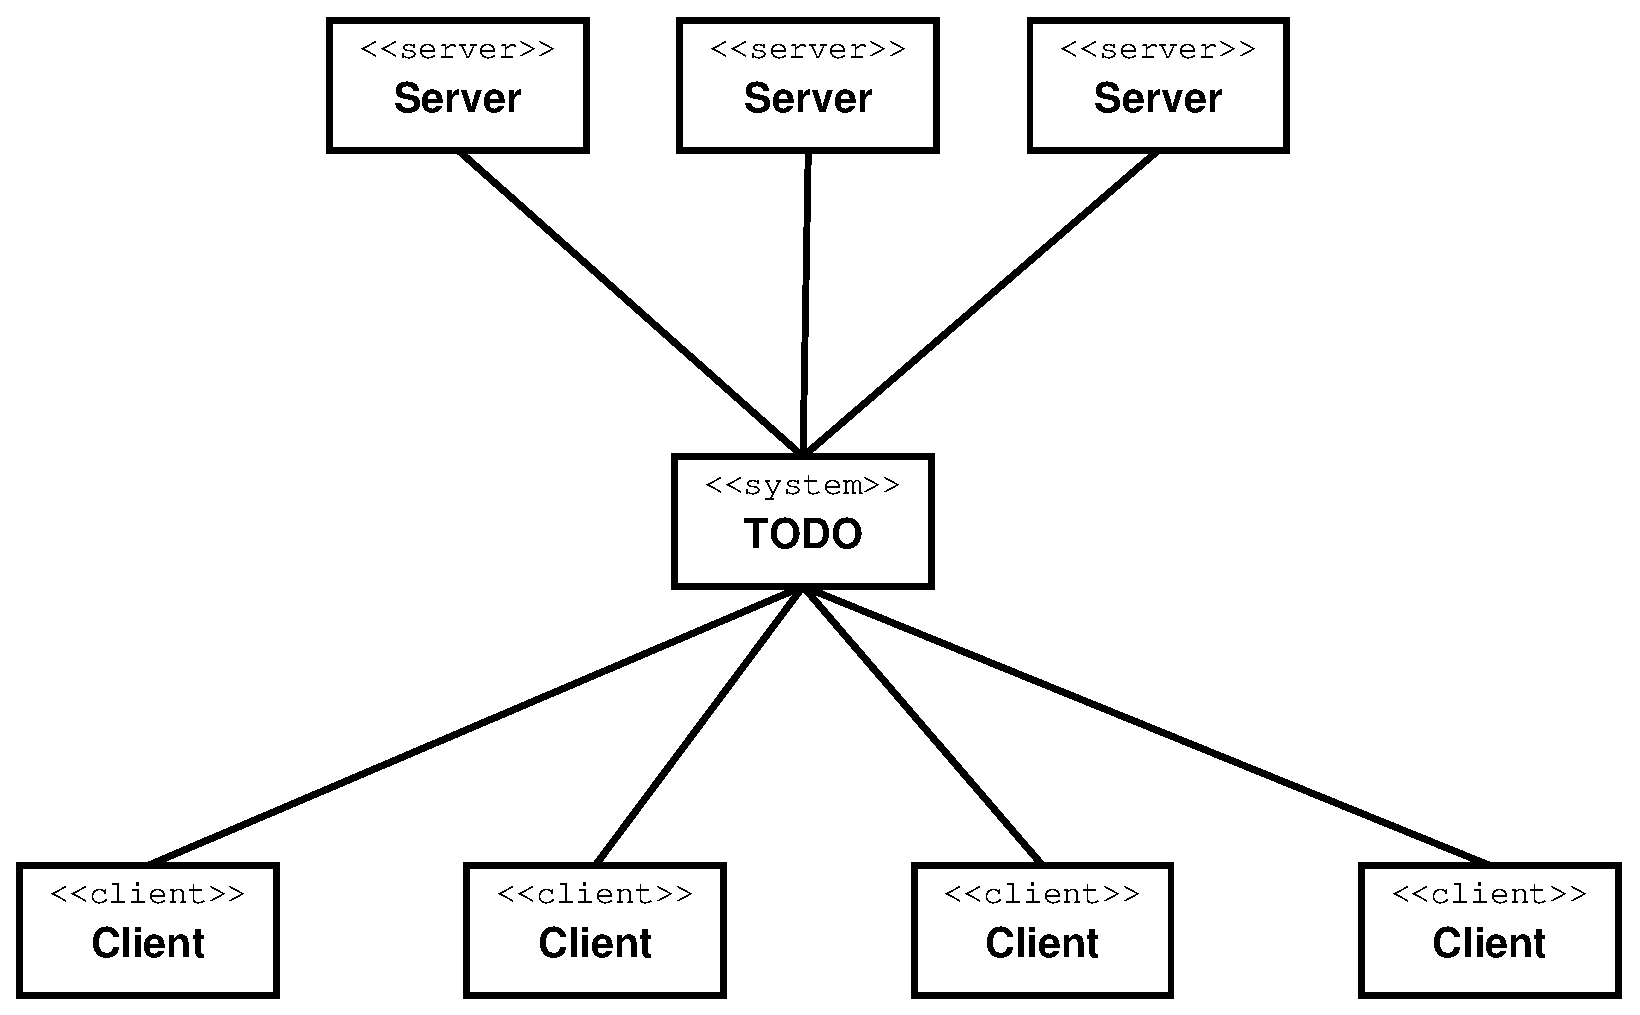
\includegraphics[width=0.7\linewidth]{Grafik/Diagramm/External}
			\caption{Externe Sicht}
			\label{fig:External}
		\end{figure}

	\end{frame}
	
	
	\section{Übersicht}
	\begin{frame}{Übersicht}
		\begin{figure}
			\centering
			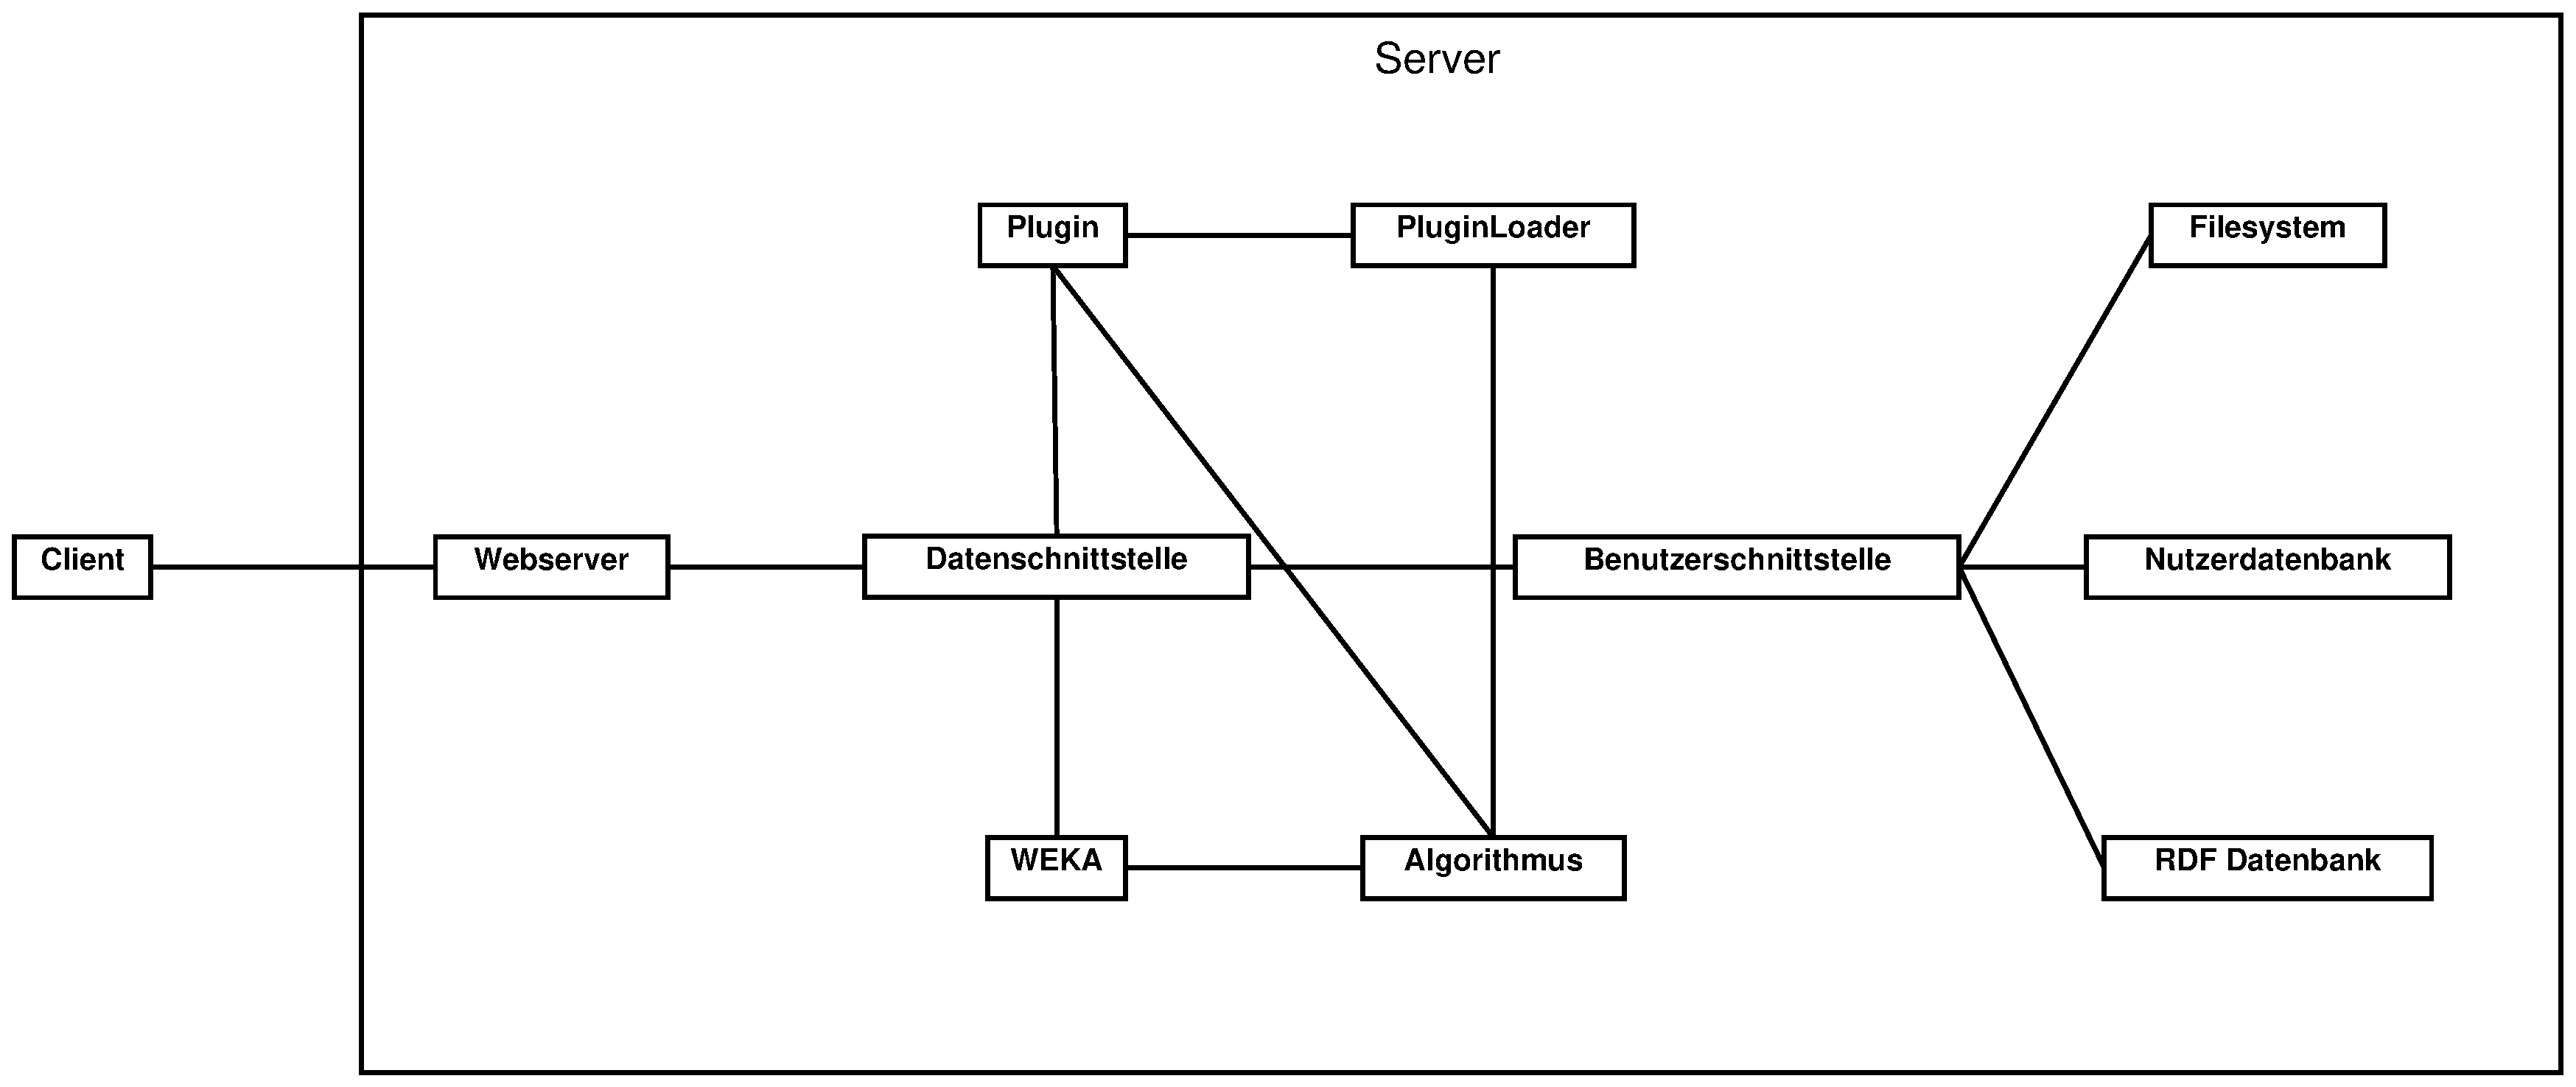
\includegraphics[width=\linewidth]{Grafik/Diagramm/Gesamt}
			\caption{Übersicht}
			\label{fig:Gesamt}
		\end{figure}
	\end{frame}
	
	\section[Struktur]{Struktur Schicht}
	\subsection{genutzte Pattern}
	\subsubsection{Client Server}
	\begin{frame}{Client Server}
		\begin{figure}
			\centering
			
\includegraphics[width=0.7\linewidth]{Grafik/Diagramm/Pattern/ClientServer/Kontext}
			\caption{Kontextdiagramm}
			\label{fig:Kontext1}
		\end{figure}
	\end{frame}
	\begin{frame}{Client Server}	
		\begin{figure}
			\centering
			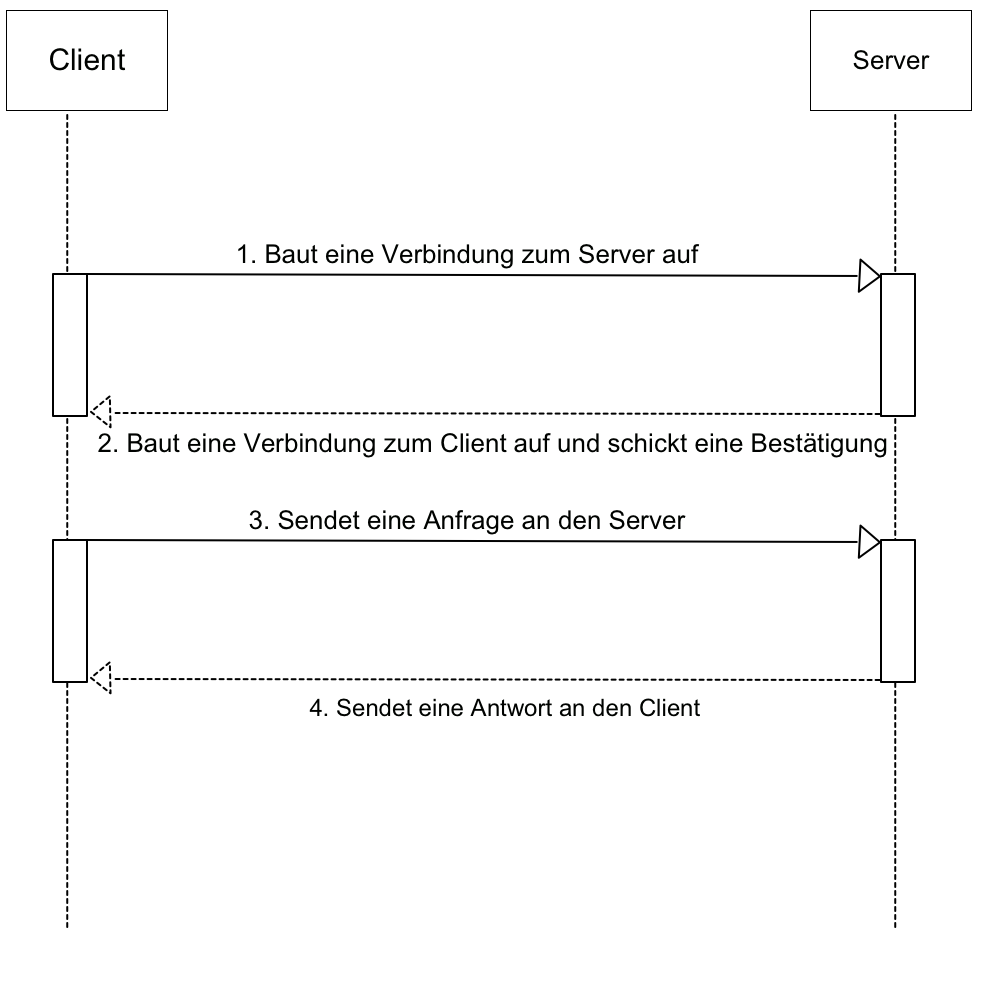
\includegraphics[height=0.8\textheight]{Grafik/Diagramm/Pattern/ClientServer/Sequenzdiagramm}
			\caption{Sequenzdiagramm}
			\label{fig:Sequenz1}
		\end{figure}
	\end{frame}
	
		\subsubsection{Microkernel}
		\begin{frame}{Microkernel}
			\begin{figure}
				\centering
				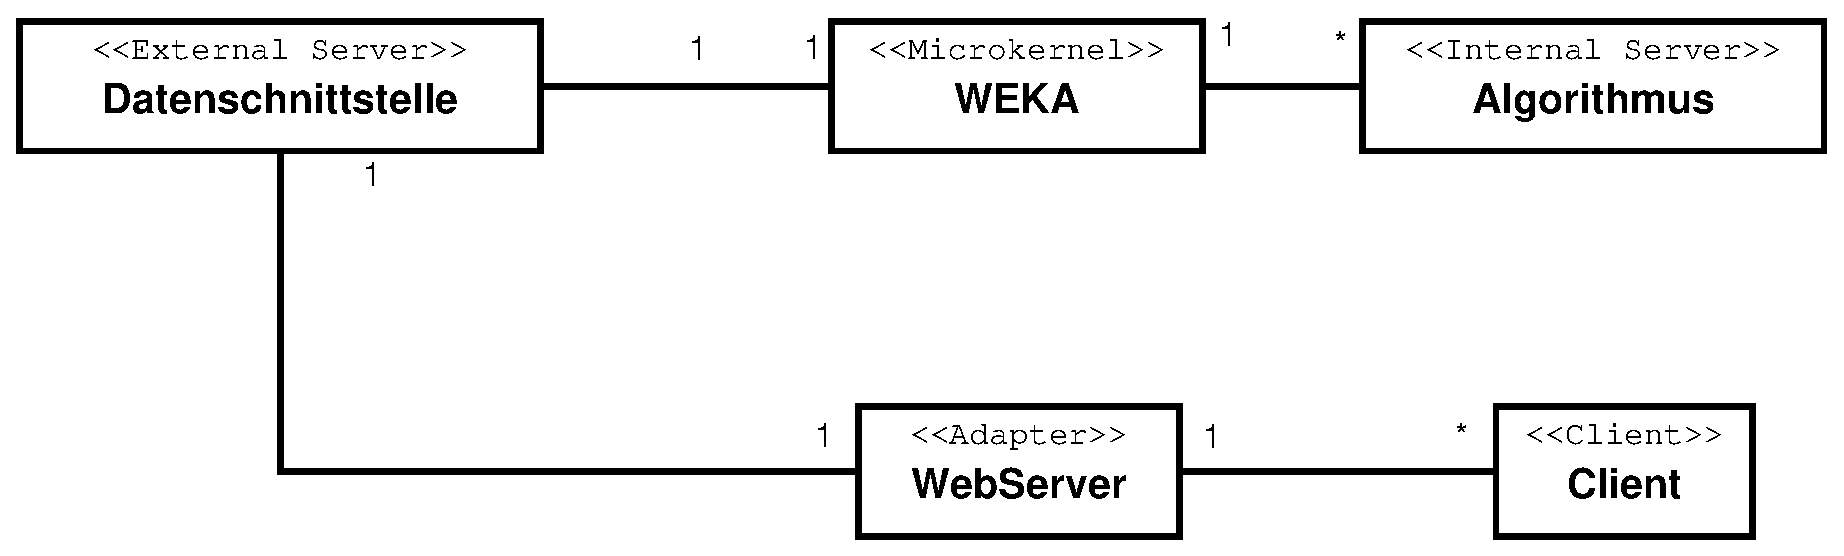
\includegraphics[width=0.7\linewidth]{Grafik/Diagramm/Microkernel}
				\caption{Kontextdiagramm}
				\label{fig:Kontext2}
			\end{figure}
		\end{frame}
		\begin{frame}{Microkernel}
			\begin{figure}[h]	
				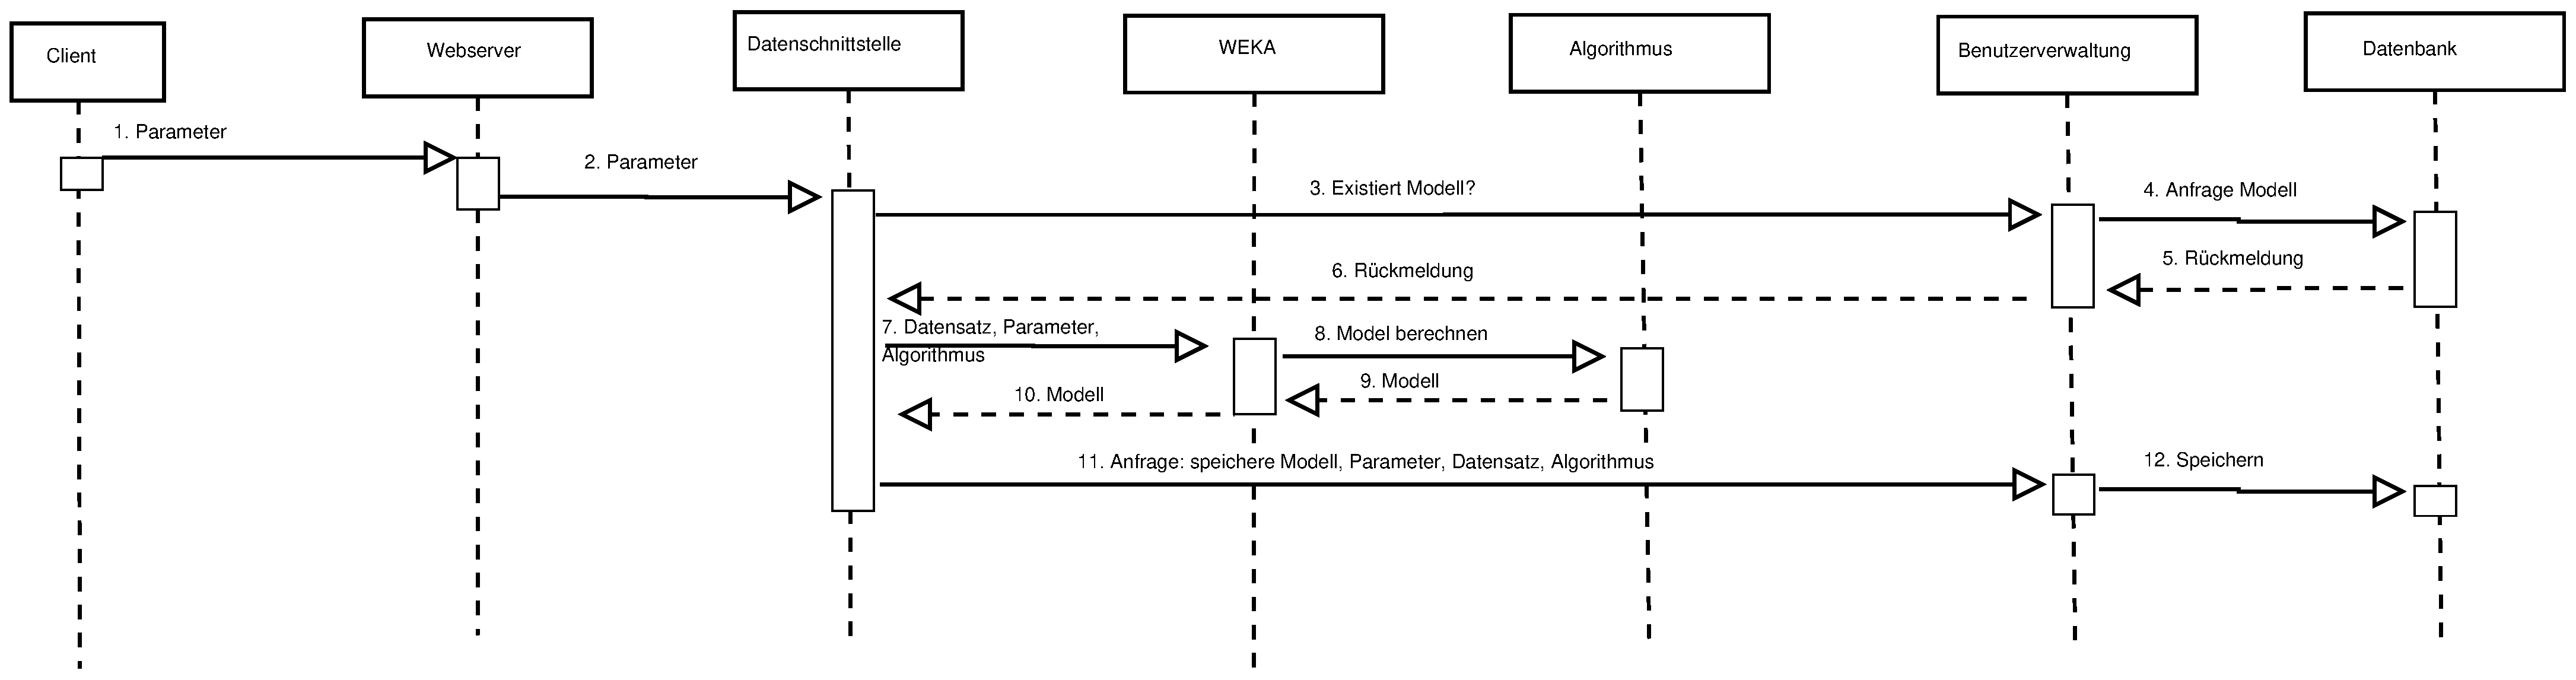
\includegraphics[width=1\linewidth]{Grafik/Diagramm/Szenarios/Berechnung3}
				\caption{Sequenzdiagramm}
				\label{fig:Sequenz2}
			\end{figure}
		\end{frame}
		
%		\subsubsection{Reflection}
%		\begin{frame}{Reflection}
%			\begin{figure}
%				\centering
%				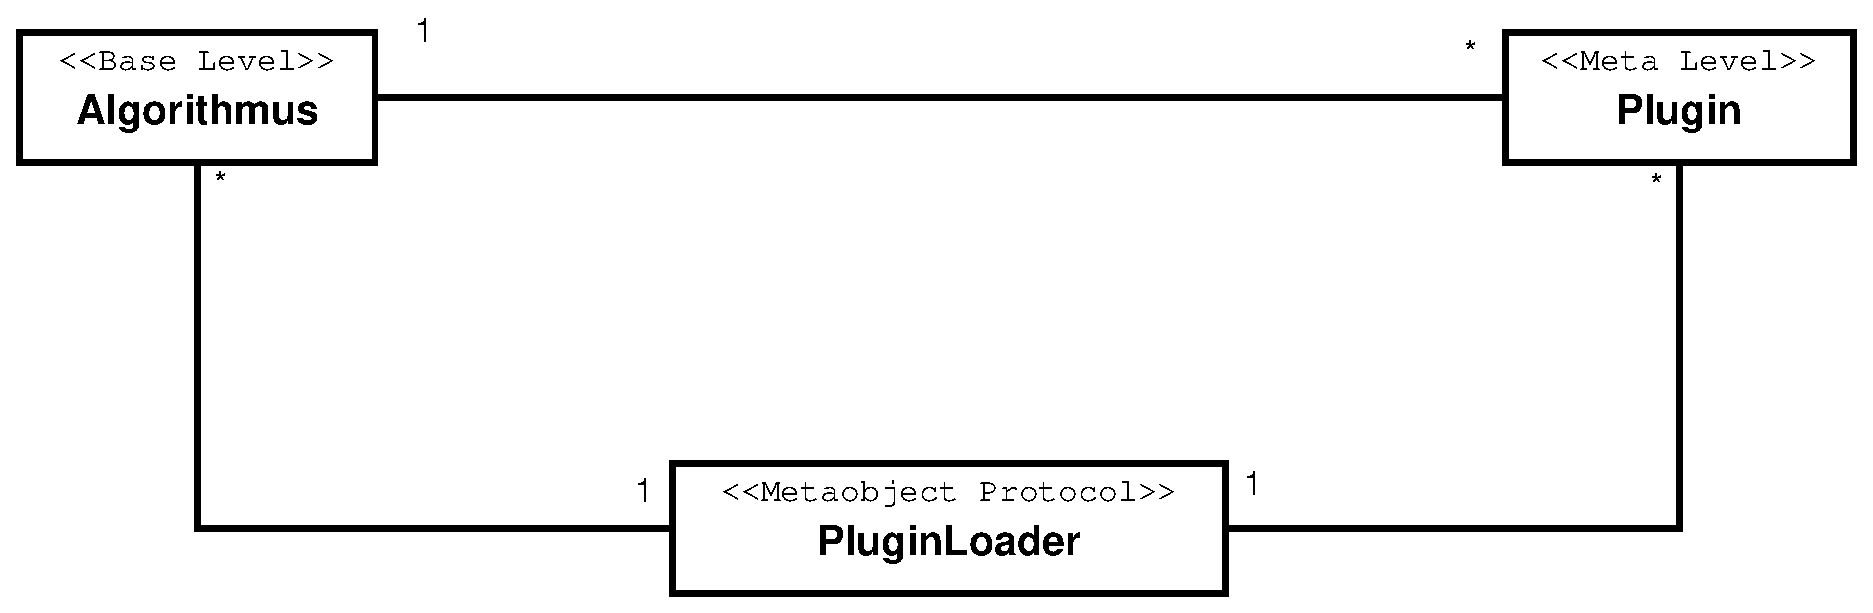
\includegraphics[width=0.7\linewidth]{Grafik/Diagramm/Reflection}
%				\caption{Kontextdiagramm}
%				\label{fig:Kontext3}
%			\end{figure}
%		\end{frame}
%		\begin{frame}{Reflection}	
%			\begin{figure}
%				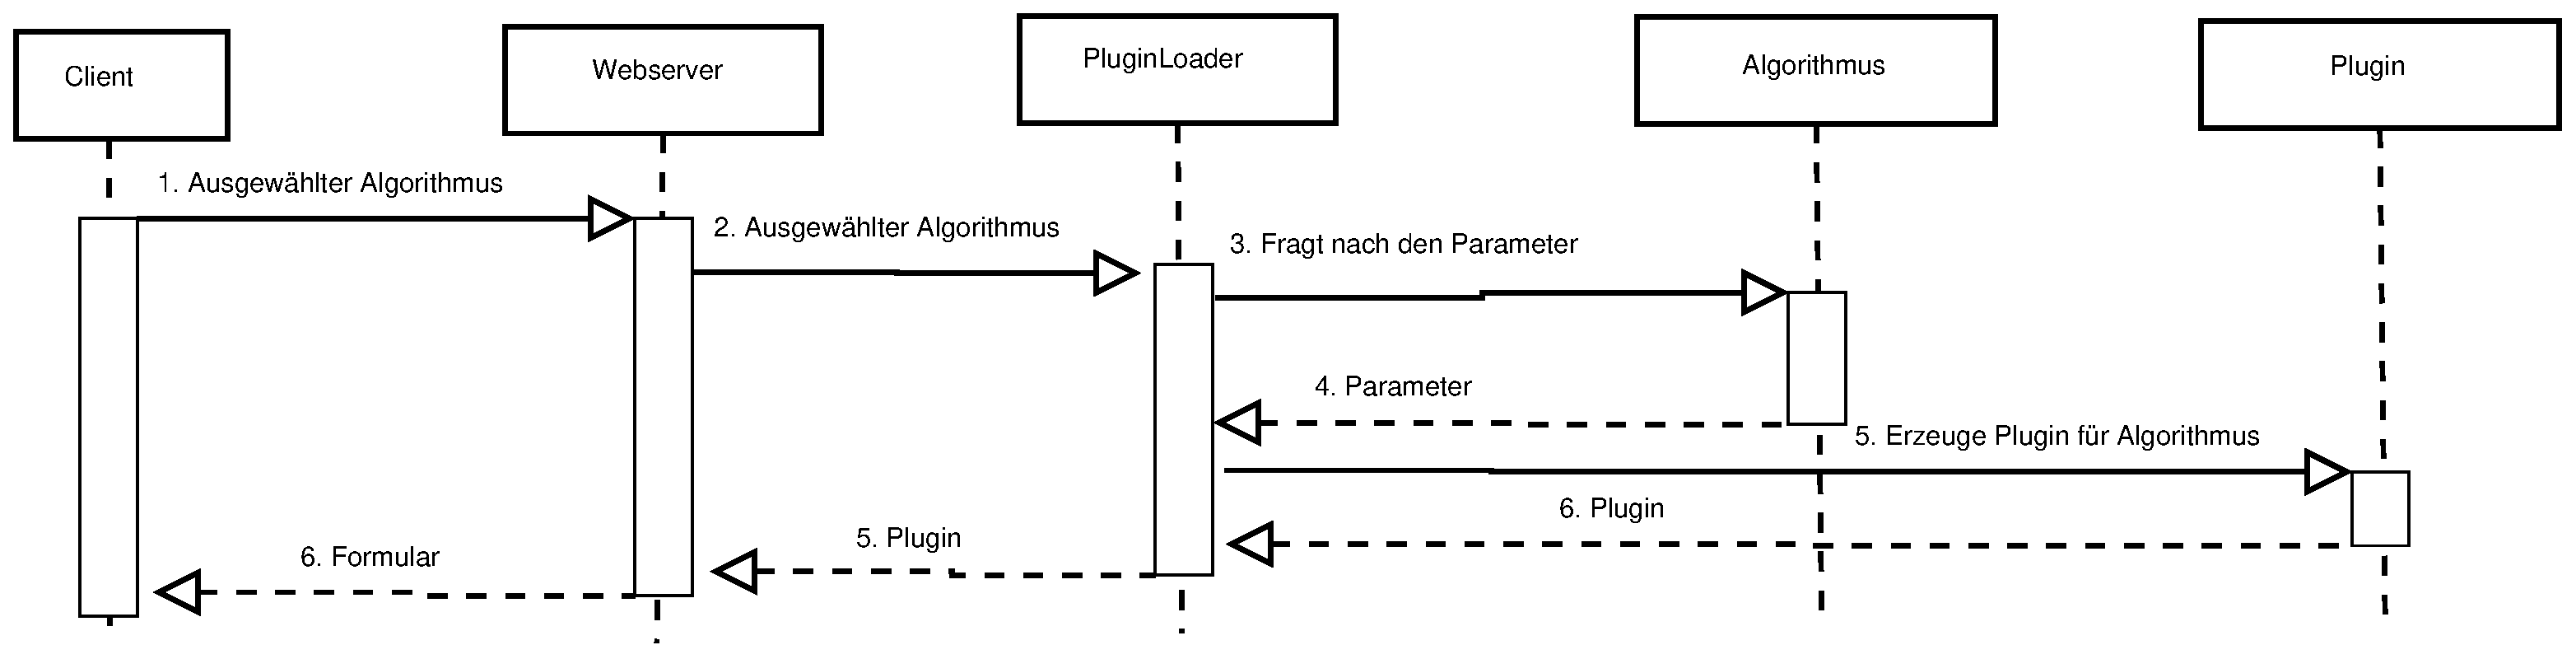
\includegraphics[width=1\linewidth]{Grafik/Diagramm/Szenarios/Berechnung2}
%				\caption{Sequenzdiagramm}
%				\label{fig:Sequenz3}
%			\end{figure}
%		\end{frame}
		
		\subsubsection{Layer}
		\begin{frame}{Layer}
			\begin{figure}
				\centering
				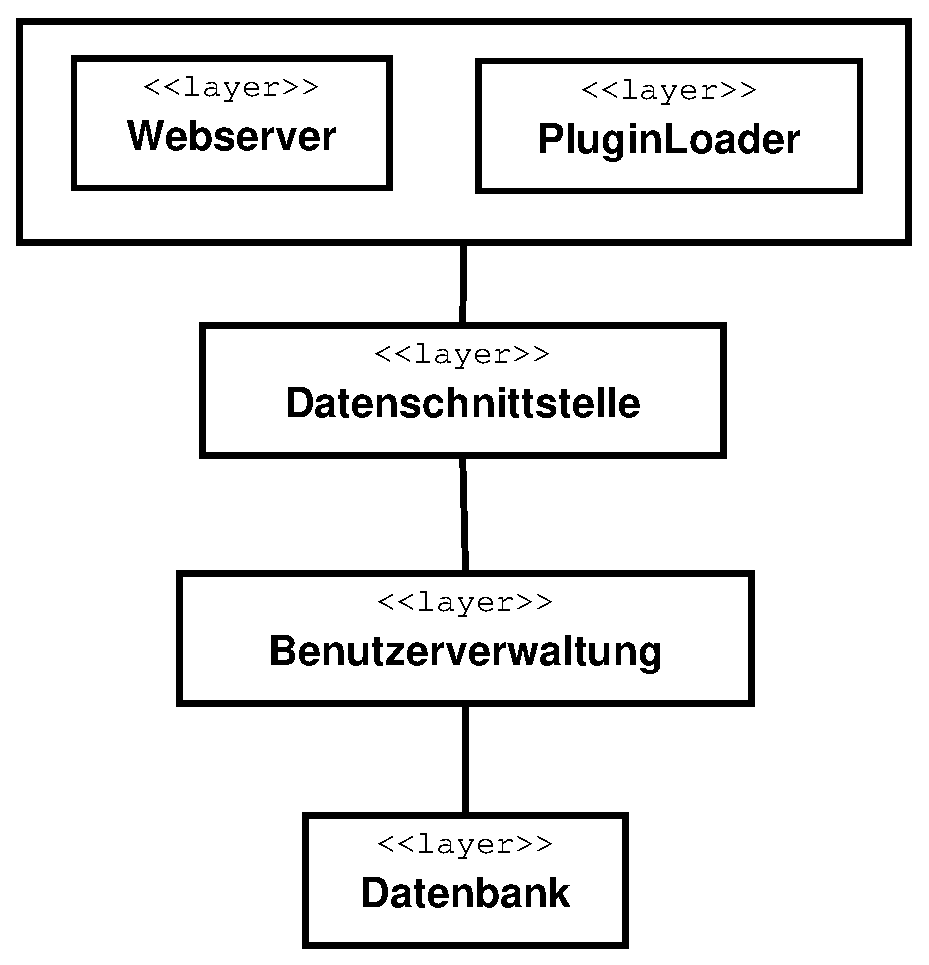
\includegraphics[height=0.8\textheight]{Grafik/Diagramm/Layer}
				\caption{Kontextdiagramm}
				\label{fig:Kontext4}
			\end{figure}
		\end{frame}
		\begin{frame}{Layer}	
			\begin{figure}
				\centering
				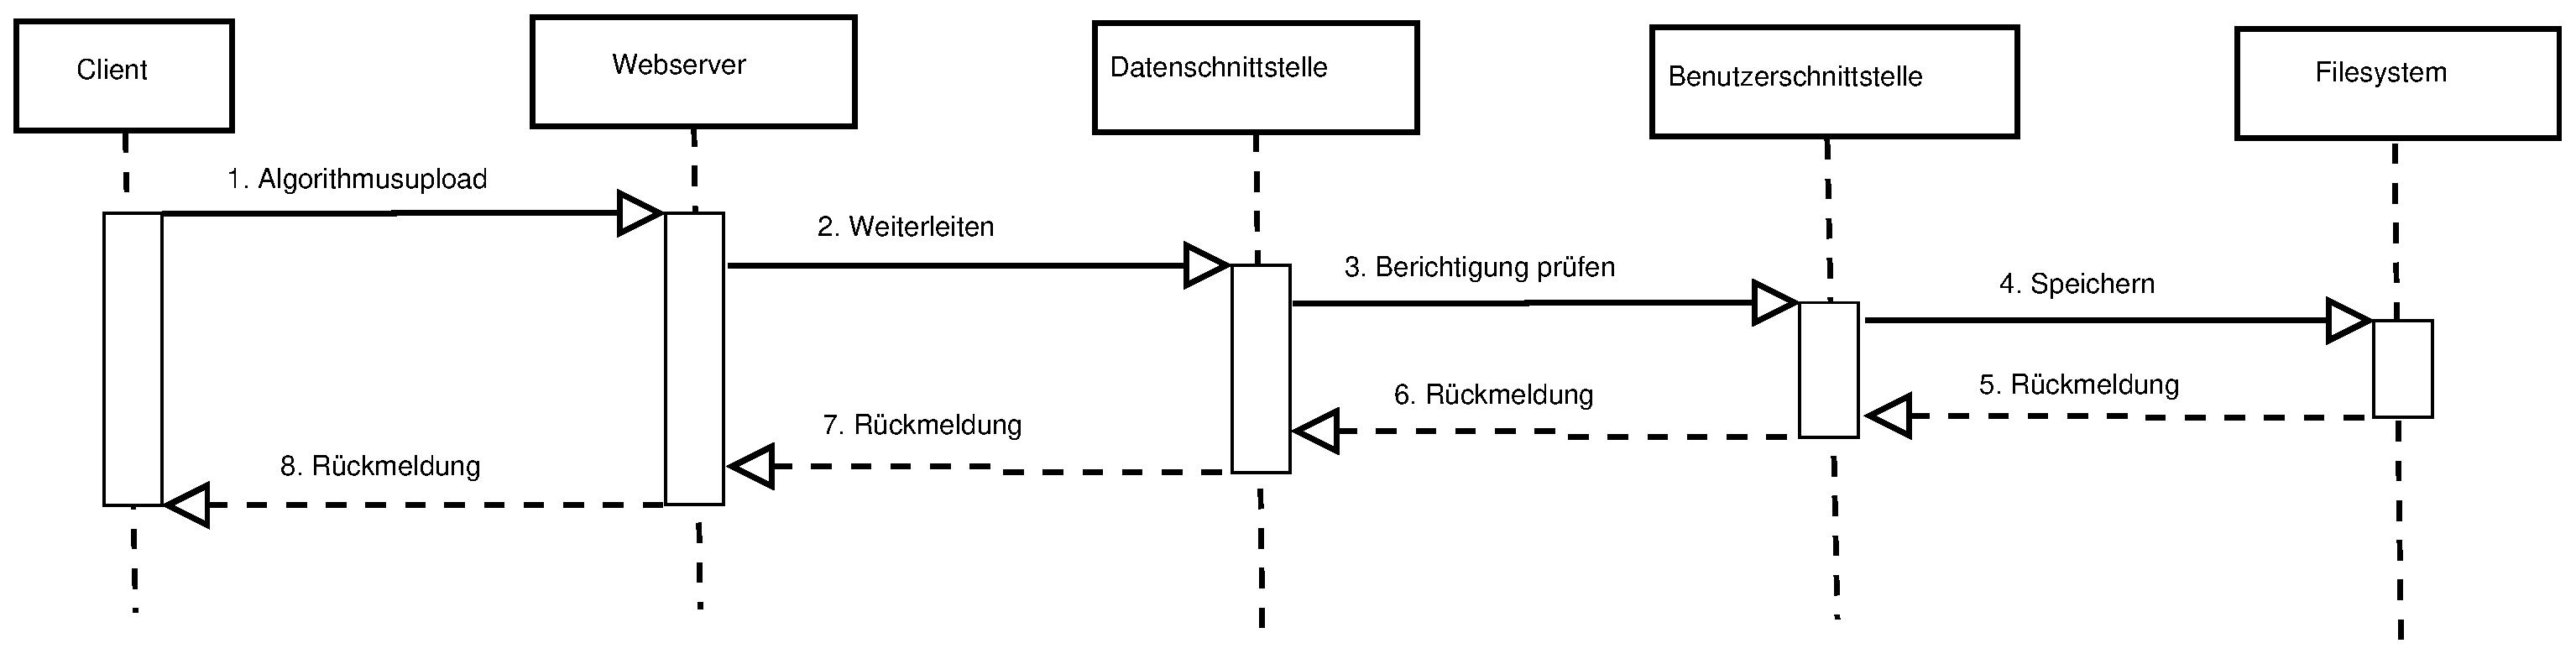
\includegraphics[width=1\linewidth]{Grafik/Diagramm/Szenarios/Algorithmus}
				\caption{Sequenzdiagramm}
				\label{fig:Sequenz4}
			\end{figure}
		\end{frame}
		
		\subsubsection[MVC]{Model-View-Controller}
		\begin{frame}{Model-View-Controller}
			\begin{figure}
				\centering
				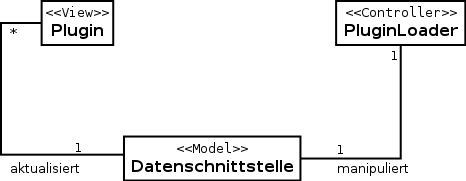
\includegraphics[width=0.7\linewidth]{Grafik/Diagramm/Pattern/MVC/Kontextdiagramm}
				\caption{Kontextdiagramm}
				\label{fig:Kontext5}
			\end{figure}
		\end{frame}
		\begin{frame}{Model-View-Controller}	
			\begin{figure}
				\centering
				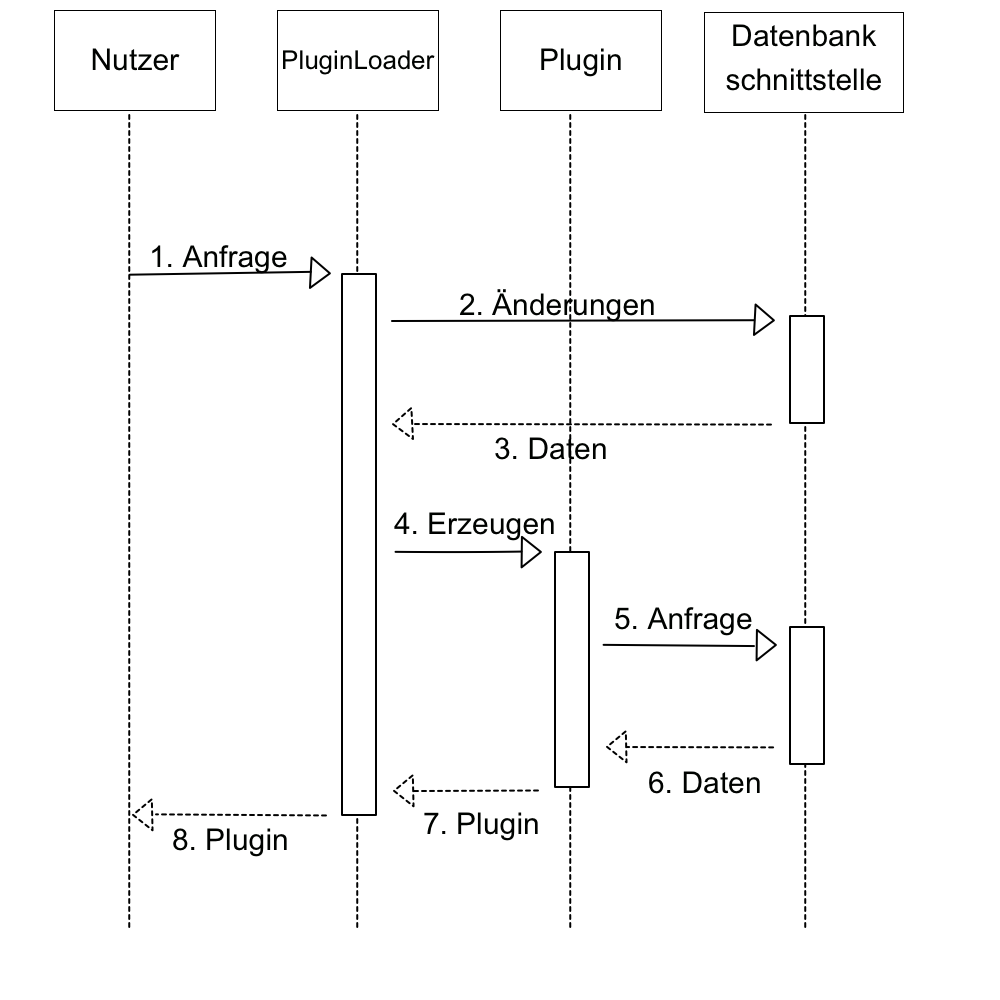
\includegraphics[height=0.8\textheight]{Grafik/Diagramm/Pattern/MVC/Sequenzdiagramm}
				\caption{Sequenzdiagramm}
				\label{fig:Sequenz5}
			\end{figure}
		\end{frame}
		
		
		\subsection{nicht genutzte Pattern}
%		\subsubsection[PAC]{Presentation-Abstraction-Control}
%		\begin{frame}{Presentation-Abstraction-Control}
%			\begin{itemize}
%				\item test
%			\end{itemize}
%		\end{frame}
		
%		\subsubsection{Pipe and Filter}
%		\begin{frame}{Pipe and Filter}
%			\begin{itemize}
%				\item test
%					
%			\end{itemize}
%		\end{frame}
%				
%		\subsubsection{Blackboard}
%		\begin{frame}{Blackboard}
%			\begin{itemize}
%				\item test
%				
%			\end{itemize}
%		\end{frame}
%		
%		\subsubsection{Broker}
%		\begin{frame}{Broker}
%			\begin{itemize}
%				\item test
%				
%			\end{itemize}
%		\end{frame}
		
		\subsubsection{Repository}
		\begin{frame}{Repository}
			\begin{itemize}
				\item single point of failur
				\item schwer zwischen mehreren Computern auszutauschen%difficult to distribute across serveral computers
				
			\end{itemize}
		\end{frame}
		
		\section[Interaktion]{Interaktionsschicht}
%		\subsection{Login}
%		\begin{frame}{Login}	
%			\begin{figure}
%				\centering
%				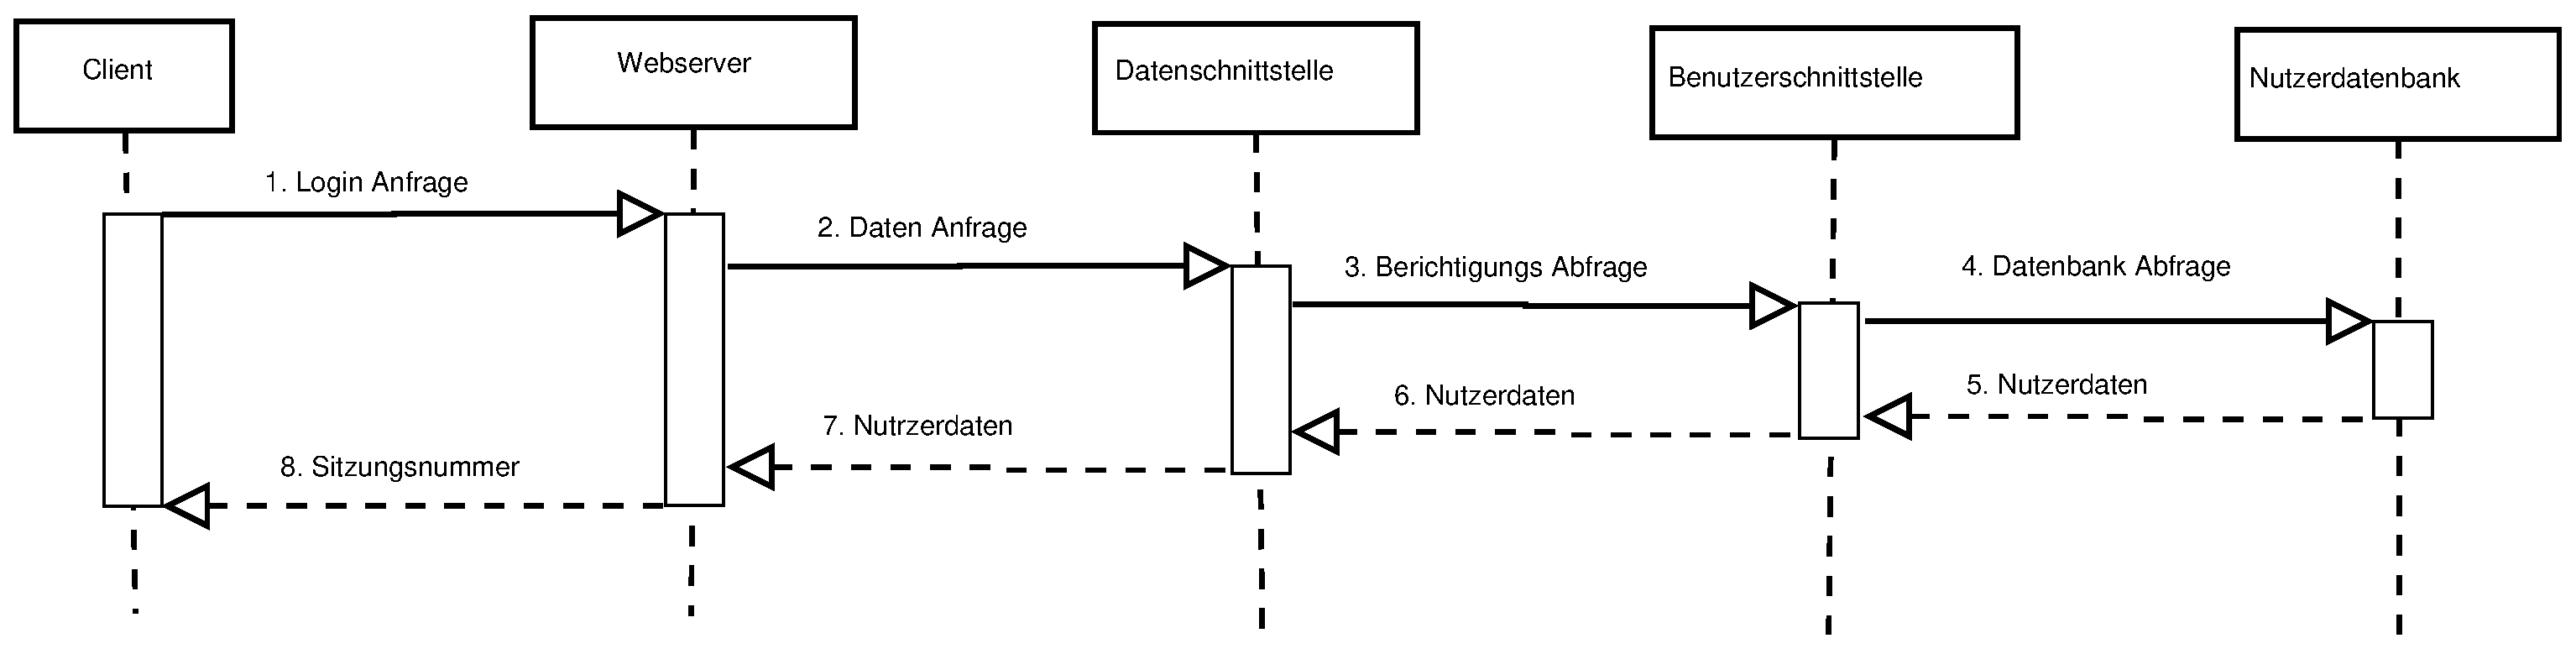
\includegraphics[width=\linewidth]{Grafik/Diagramm/Szenarios/Login}
%				\caption{Login}
%				\label{fig:Login}
%			\end{figure}
%		\end{frame}
%		
%		\subsection{Algorithmus hinzufügen}
%		\begin{frame}{Algorithmus hinzufügen}	
%			\begin{figure}
%				\centering
%				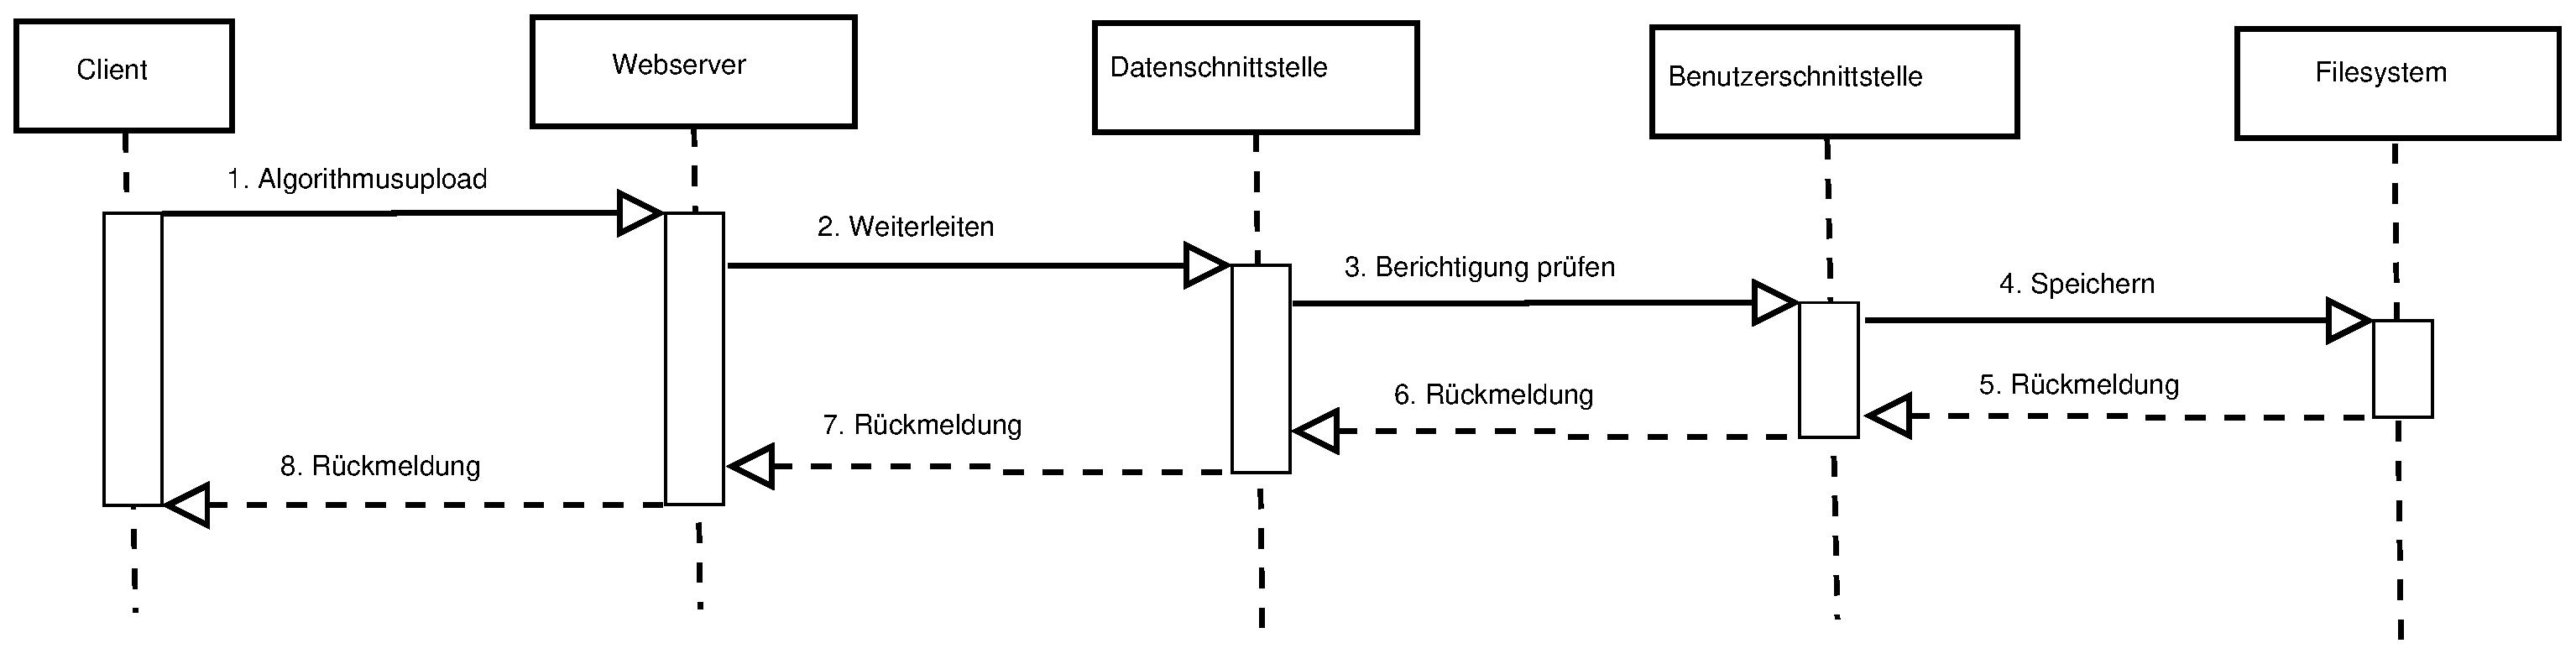
\includegraphics[width=\linewidth]{Grafik/Diagramm/Szenarios/Algorithmus}
%				\caption{Algorithmus hinzufügen}
%				\label{fig:Algorithmus}
%			\end{figure}
%		\end{frame}
		
		\subsection[Berechnung]{Berechnung eines Modells}
		\begin{frame}{Berechnung eines Modells}	
			\begin{figure}
				\centering
				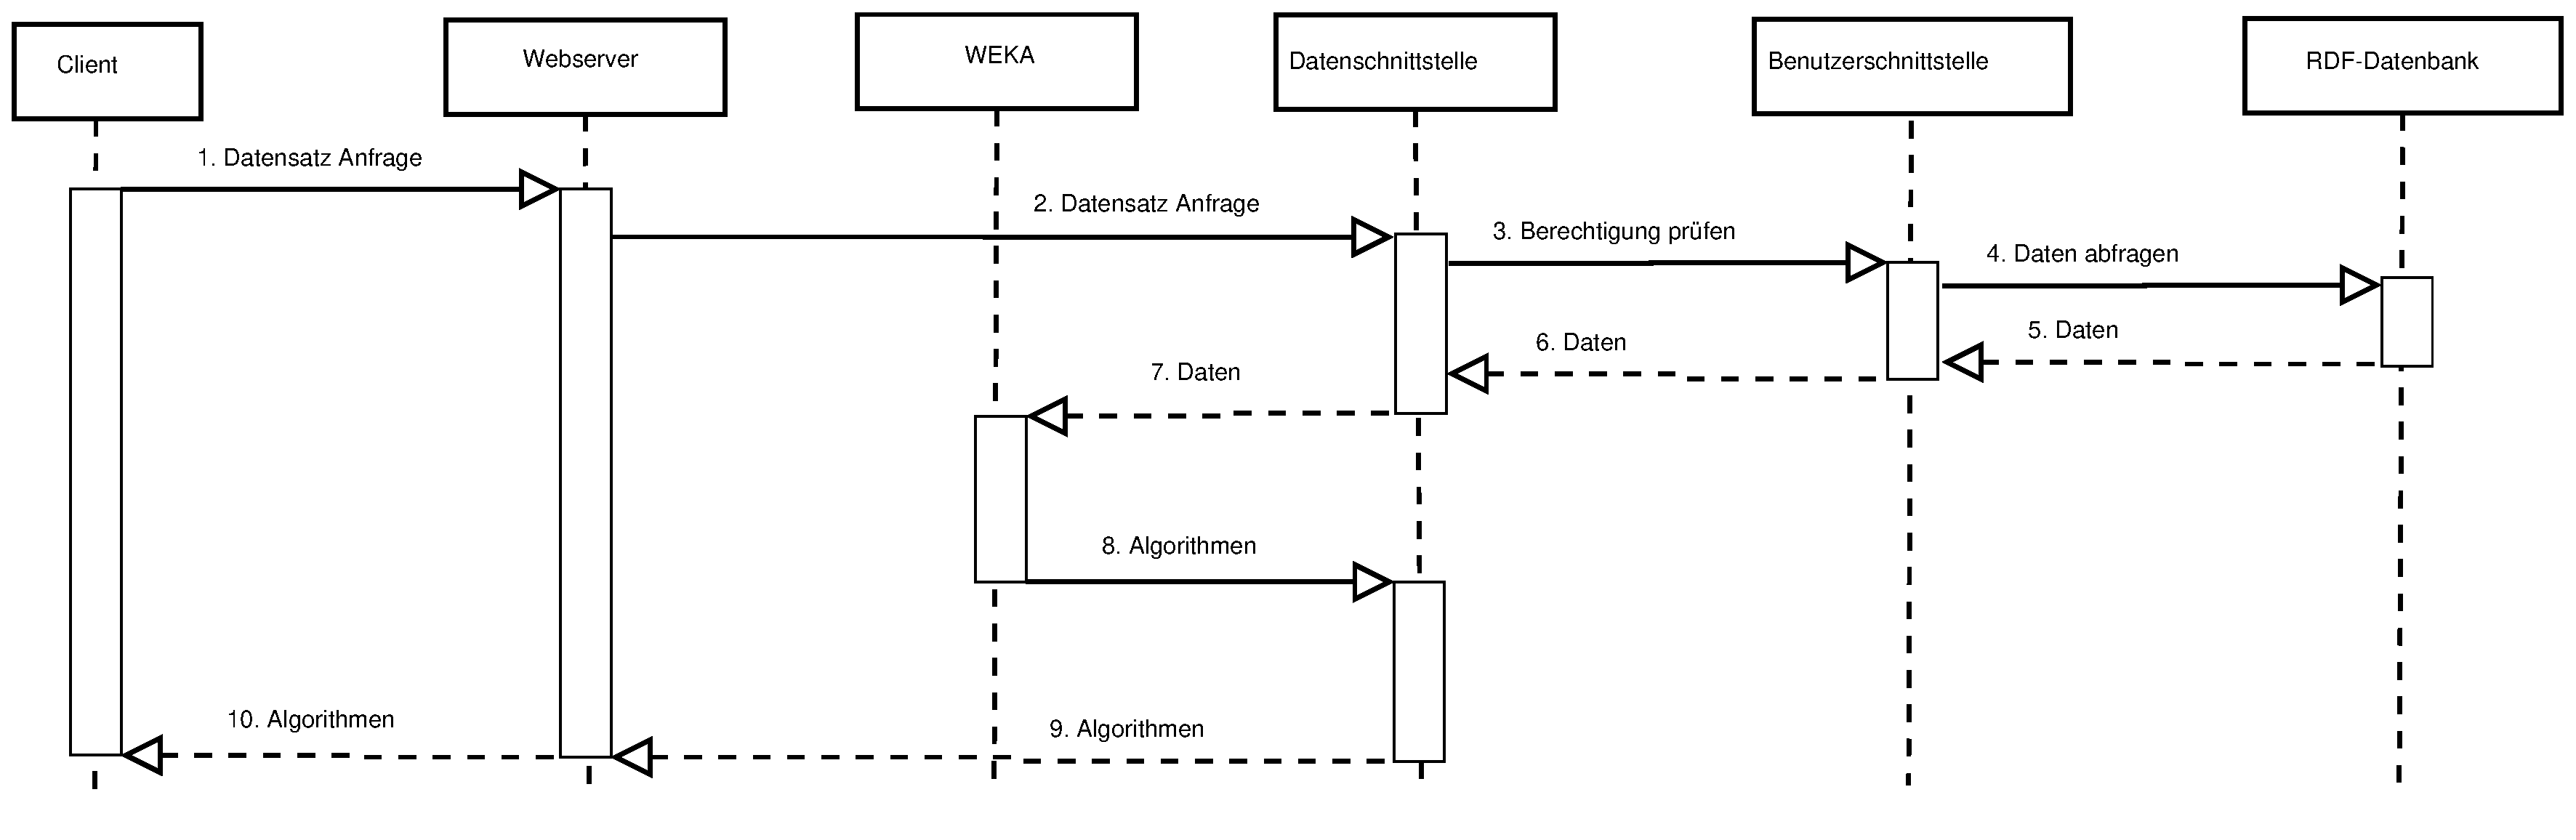
\includegraphics[width=\linewidth]{Grafik/Diagramm/Szenarios/Berechnung}
				\caption{Berechnung eines Modells 1}
				\label{fig:Berechnung1}
			\end{figure}
		\end{frame}
		\begin{frame}{Berechnung eines Modells}	
			\begin{figure}
				\centering
				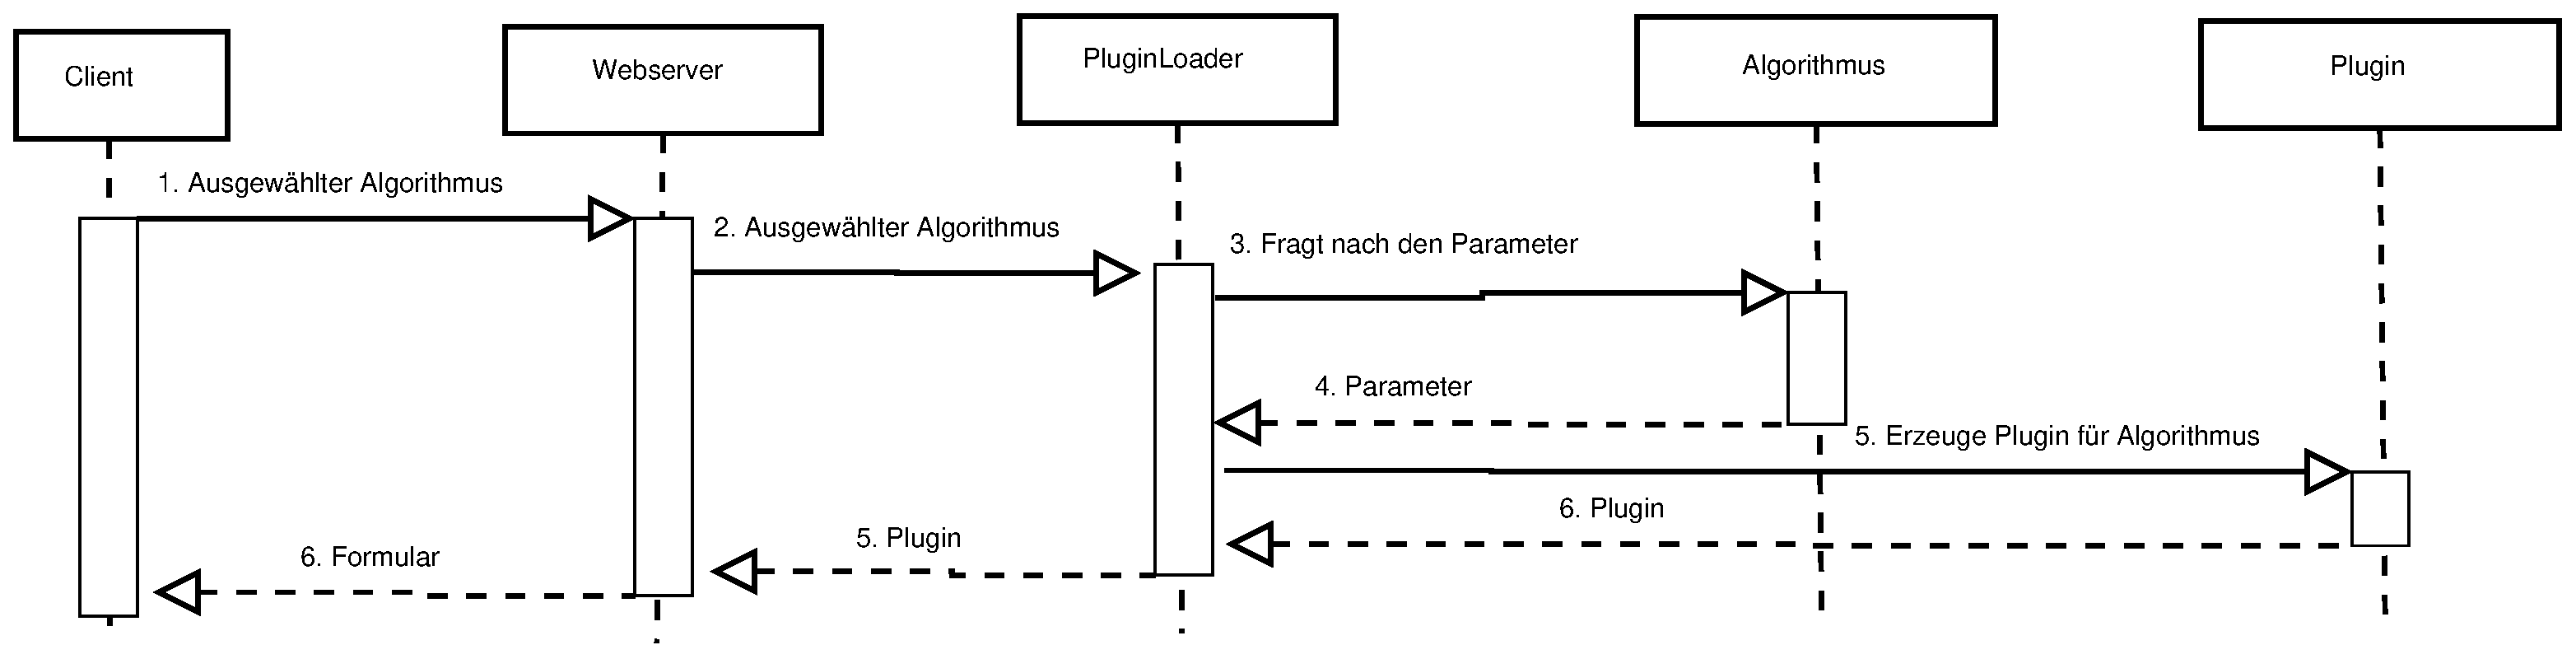
\includegraphics[width=\linewidth]{Grafik/Diagramm/Szenarios/Berechnung2}
				\caption{Berechnung eines Modells 2}
				\label{fig:Berechnung2}
			\end{figure}
		\end{frame}
		\begin{frame}{Berechnung eines Modells}	
			\begin{figure}
				\centering
				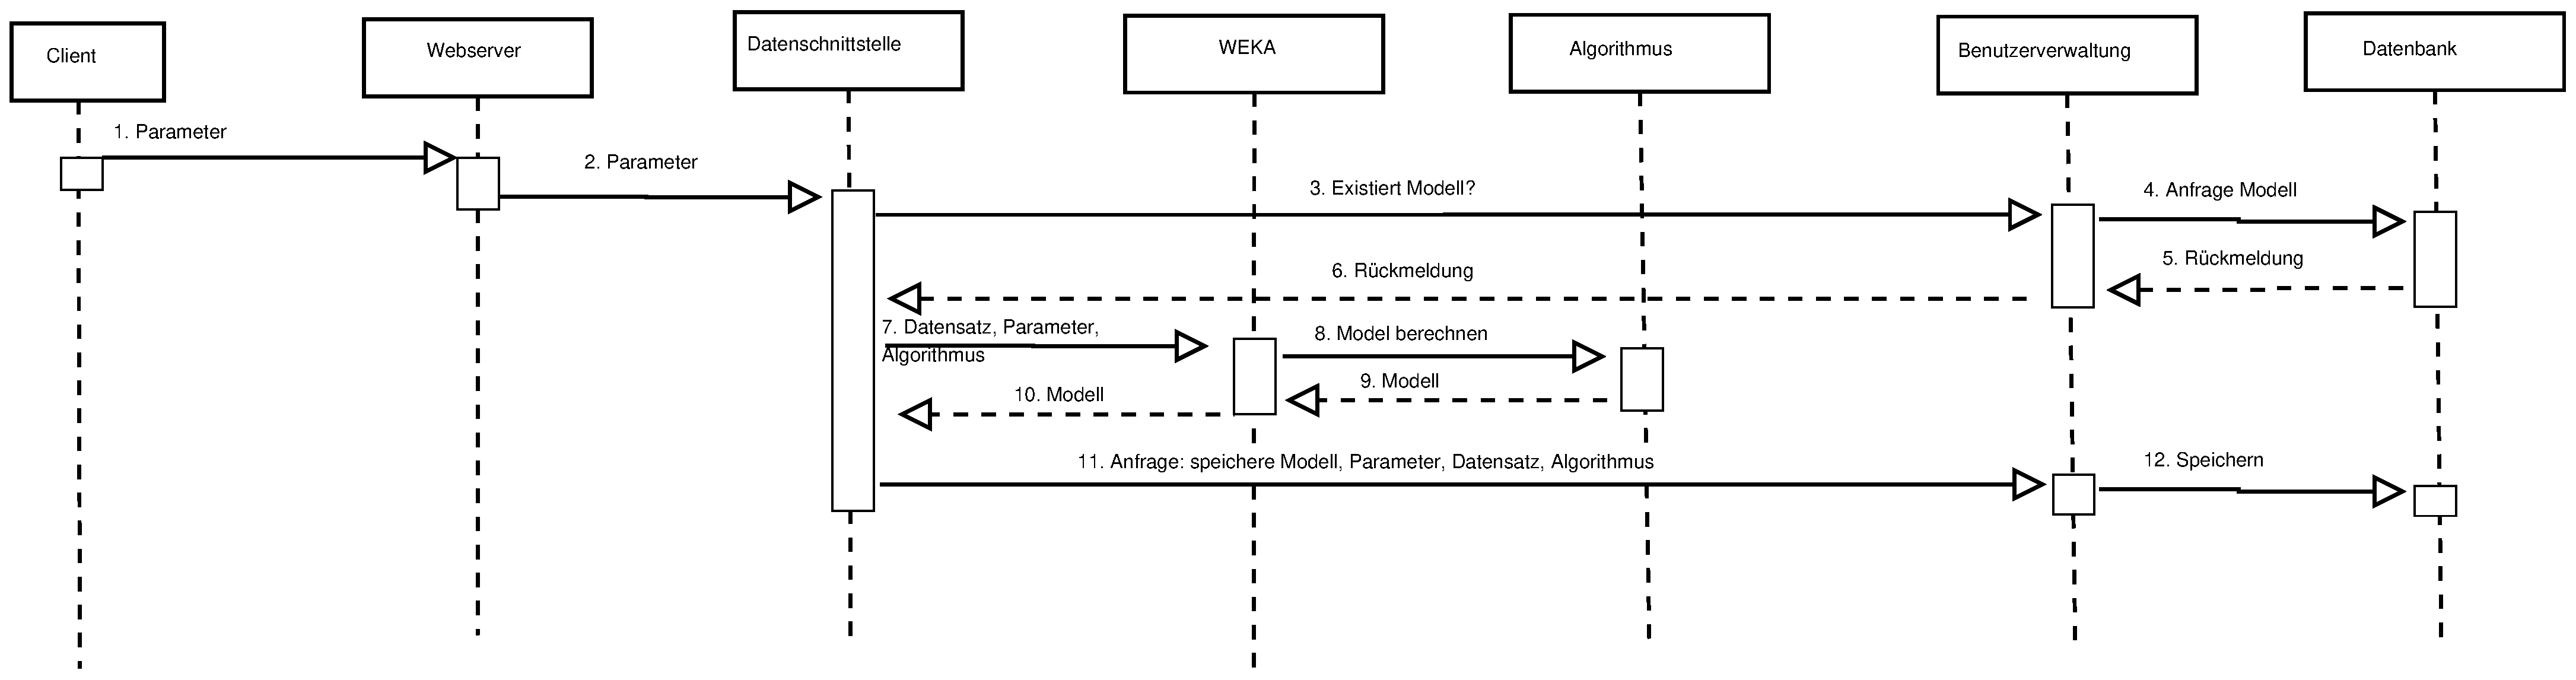
\includegraphics[width=\linewidth]{Grafik/Diagramm/Szenarios/Berechnung3}
				\caption{Berechnung eines Modells 3}
				\label{fig:Berechnung3}
			\end{figure}
		\end{frame}	
		
\end{document}